%% evaluating_orthologue_prediction.tex
%% Author: Leighton Pritchard
%% Copyright: James Hutton Institute
%% A brief introduction to orthologues, and evaluation of their prediction

% SUBSECTION: Why orthologues?
\subsection{Evaluating orthologue prediction}

% Which methods work best
\begin{frame}
  \frametitle{Which prediction methods work best?
    \footnote{\tiny{Wolf and Koonin (2012) \textit{Genome Biol. Evol.} \textbf{4}:1286-1294 \href{http://dx.doi.org/10.1093/gbe/evs100}{doi:10.1093/gbe/evs100
    }}}
  }
  Taking advantage of prokaryotic operon structure: \textcolor{RawSienna}{\textbf{if the outer pair of a syntenic triplet of genes are orthologous, the middle gene is also likely to be orthologous}.}\\
  Specifically testing reciprocal best hits (RBH).
  \begin{center}
      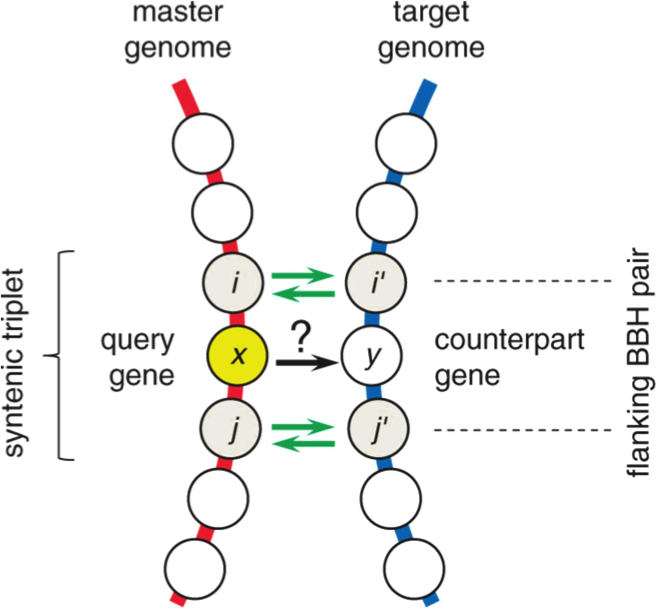
\includegraphics[height=0.45\textheight]{images/syntenic_triplet} 
  \end{center}
\end{frame}

% Which methods work best
\begin{frame}
  \frametitle{Which prediction methods work best?
    \footnote{\tiny{Wolf and Koonin (2012) \textit{Genome Biol. Evil.} \textbf{4}:1286-1294 \href{http://dx.doi.org/10.1093/gbe/evs100}{doi:10.1093/gbe/evs100
    }}}
  }
  \begin{itemize}
    \item \textcolor{hutton_green}{Tested on 573 prokaryotic genomes}
    \item \textcolor{hutton_blue}{88-99\% of RBH found in syntenic triplets}
    \item \textcolor{hutton_purple}{Overwhelming majority of middle genes are RBH}
  \end{itemize}
  \textcolor{red}{\textbf{RBH reliably finds ``orthologues''.}}
  \begin{center}
      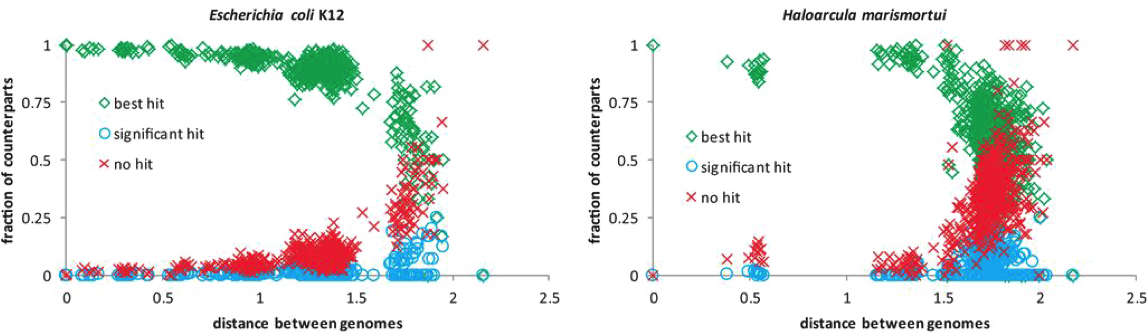
\includegraphics[width=1\textwidth]{images/syntenic_triplet_results} 
  \end{center}
\end{frame}

% Which methods work best
\begin{frame}
  \frametitle{Which prediction methods work best?
    \footnote{\tiny{Salichos and Rokas (2011) \textit{PLoS One} \textbf{6}:e18755 \href{http://dx.doi.org/10.1371/journal.pone.0018755.g006}{doi:10.1371/journal.pone.0018755.g006
  }}}
  }
  Four methods tested against 2,723 curated orthologues from six \textit{Saccharomycetes}
  \begin{itemize}
    \item \textcolor{hutton_green}{RBBH (and cRBH); RSD (and cRSD); MultiParanoid; OrthoMCL}
    \item \textcolor{hutton_blue}{Rated by statistical performance metrics: sensitivity, specificity, accuracy, FDR}
  \end{itemize}
  \textcolor{hutton_purple}{\textbf{cRBH most accurate and specific, with lowest FDR.}}
  \begin{center}
      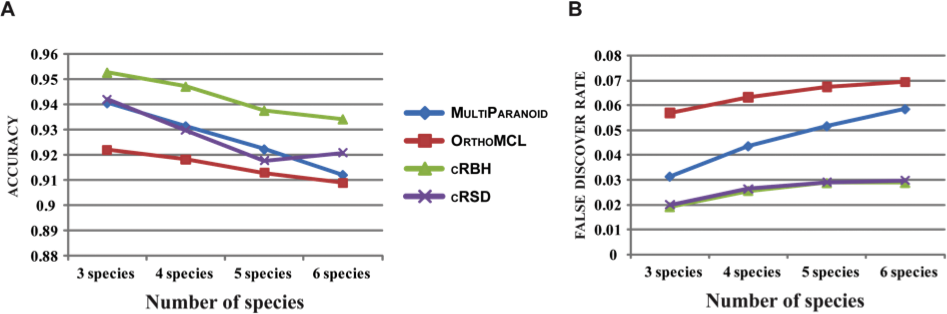
\includegraphics[height=0.25\textheight]{images/salichos_results1} 
      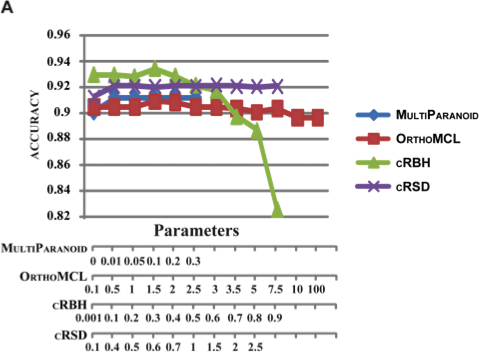
\includegraphics[height=0.25\textheight]{images/salichos_results2}      
  \end{center}
\end{frame}

% Which methods work best
\begin{frame}
  \frametitle{Which prediction methods work best?
    \footnote{\tiny{Altenhoff and Dessimoz (2009) \textit{PLoS Comp. Biol.} \textbf{5}:e1000262 \href{http://dx.doi.org/10.1371/journal.pcbi.1000262}{doi:10.1371/journal.pcbi.1000262
    }}}
  }
  Testing on literature-based benchmarks for grouping by function and correct branching of phylogeny.  \begin{center}
      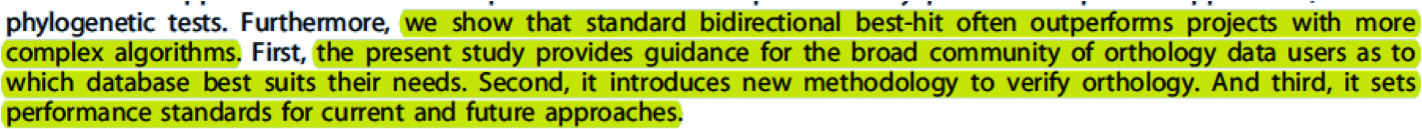
\includegraphics[width=1\textwidth]{images/altenhoff1} \\
      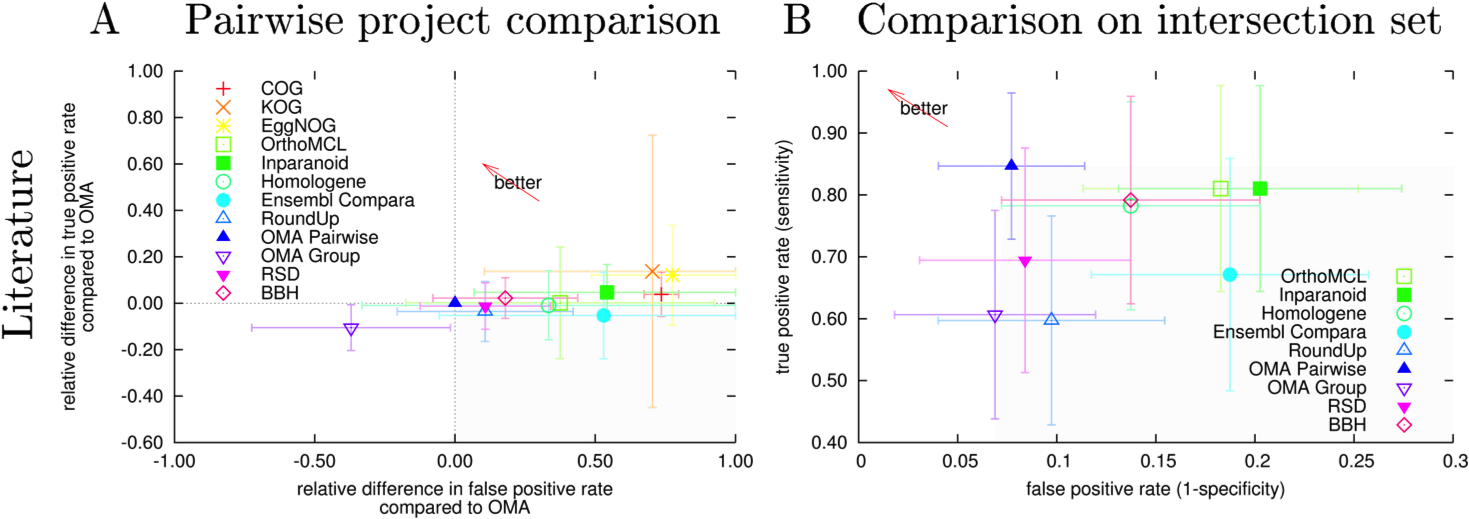
\includegraphics[width=1\textwidth]{images/altenhoff2}      
  \end{center}
\end{frame}

% Which methods work best
\begin{frame}
  \frametitle{Which prediction methods work best?}
  \begin{itemize}
    \item \textcolor{hutton_green}{Performance varies by choice of method, and interpretation of ``orthology''}
    \item \textcolor{hutton_blue}{Biggest influence is genome annotation quality}
    \item Relative performance varies with choice of benchmark
    \item \textcolor{hutton_purple}{\textbf{(clustering) RBH outperforms more complex algorithms under many circumstances}}
  \end{itemize}
\end{frame}

% Which methods work best
\begin{frame}
  \frametitle{What is this magic RBH method?}
  \begin{center}
      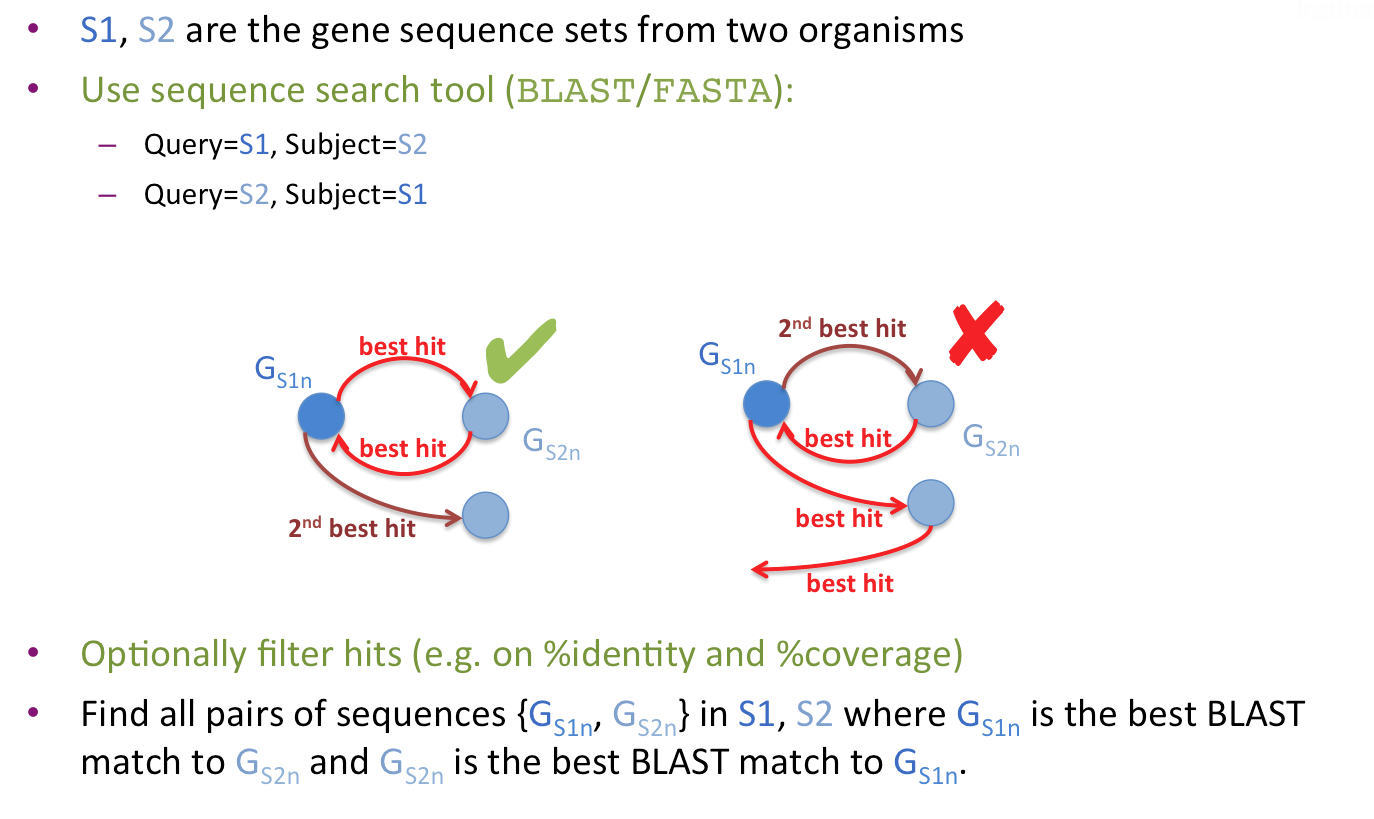
\includegraphics[width=1\textwidth]{images/rbbh}      
  \end{center}
\end{frame}

%
\begin{frame}
  \frametitle{Finding ``Orthologues'': RBBH}
  \Large{
    \textcolor{hutton_blue}{
      \textbf{
      EXERCISE 8: \\
      \texttt{find\_rbbh/ex08\_find\_rbbh.ipynb}
      }
    }
  }
\end{frame}

%
\begin{frame}
  \frametitle{Finding ``Orthologues'': MCL}
  \Large{
    \textcolor{hutton_blue}{
      \textbf{
      EXERCISE 9: \\
      {\small \href{https://github.com/widdowquinn/Teaching-2015-03-17-UoD_compgenvis/blob/master/exercises/mcl_orthologues/ex09a_mcl_orthologues.md}{\texttt{mcl\_orthologues/ex\_09a\_mcl\_orthologues.md}} \\
      \texttt{mcl\_orthologues/ex09b\_mcl\_orthologues.ipynb}}
      }
    }
  }
\end{frame}